\documentclass[
onecolumn,
superscriptaddress,
longbibliography,
nofootinbib,
 amsmath,amssymb,
 aps,
prb
]{revtex4-2}


\usepackage{lipsum}
\usepackage{caption}
\usepackage[normalem]{ulem}
\usepackage{dsfont}
\usepackage{float}
\usepackage{wasysym}
\usepackage{cancel}
\usepackage{braket}
\usepackage{physics}
\usepackage{comment}

\usepackage[dvipsnames]{xcolor}
\usepackage{appendix}
\usepackage{caption}
\usepackage{enumerate}
\captionsetup{justification=raggedright,singlelinecheck=false}
\usepackage{subcaption}
\usepackage{graphicx}% Include figure files
\graphicspath{ {./images_response/} }
\usepackage{dcolumn}% Align table columns on decimal point
\usepackage[mathscr]{euscript}
\usepackage[scr=boondox]{mathalpha}
\usepackage{bm}% bold math
\usepackage[linktocpage]{hyperref}% add hypertext capabilities
\hypersetup{colorlinks=true,citecolor=blue,linkcolor=blue, urlcolor=blue, breaklinks=true}
%\usepackage[mathlines]{lineno}% Enable numbering of text and display math
%\linenumbers\relax % Commence numbering lines
% \usepackage{booktabs}
% % \usepackage{textcomp, complexity}
% \usepackage{times}


\newcommand{\commentGN}[1]{{\color{purple}\footnotesize{GN: #1}}}
\newcommand{\commentJS}[1]{\textcolor{blue}{\footnotesize{JS: #1}}}
\newcommand{\response}[1]{\textcolor{Mulberry}{#1}}

\newcommand{\vS}{\vec{S}}
\newcommand{\utop}{\ensuremath{U(1)_{\text{top}}}}
\newcommand{\chiof}[3]{\ensuremath{(\hat{\va{S}}_{#1}\cross \hat{\va{S}}_{#2})\vdot \hat{\va{S}}_{#3}}}
\newcommand{\Sof}[1]{\ensuremath{\hat{\va{S}}_{#1}}}
\newcommand{\crossof}[2]{\ensuremath{\hat{\va{S}}_{#1}\cross \hat{\va{S}}_{#2}}}
\newcommand{\dotof}[2]{\ensuremath{\hat{\va{S}}_{#1}\vdot \hat{\va{S}}_{#2}}}
\newcommand{\parchi}[4]{\ensuremath{\hat{\vb{S}}_{#1}^{#4}(\crossof{#2}{#3})^{#4}}}
\newcommand{\upnchi}{\ensuremath{\hat{\chi}_{\triangle,\vec{n}}}}
\newcommand{\downnchi}{\ensuremath{\hat{\chi}_{\triangledown,\vec{n}}}}
\newcommand{\Upchi}[2]{\ensuremath{\chi_{\triangle,\vb{n}+(#1,#2)}}}
\newcommand{\Downchi}[2]{\ensuremath{\chi_{\triangledown,\vb{n}+(#1 , #2)}}}
\newcommand\bdot[1][.5]{\mathbin{\vcenter{\hbox{\scalebox{#1}{$\bullet$}}}}}
\newcommand{\mysymb}[2]{\mathord{\vcenter{\hbox{\includegraphics[height=#2 ex]{#1}}}}}
\newcommand{\Z}{\mathbb{Z}}
\newcommand{\Tm}{\hat{\mathcal{T}}_R}
\newcommand{\tnew}{\mathrm{t}}
\newcommand{\tot}[1]{#1_{\mathrm{tot}}}
\newcommand{\dual}[1]{\boldsymbol{\mathsf{#1}}}

\renewcommand\thefigure{R\arabic{figure}}   

\makeatletter
\newcommand\xlabel[2][]{\phantomsection\def\@currentlabelname{#1}\label{#2}}
\makeatother
%\usepackage[showframe,%Uncomment any one of the following lines to test 
%%scale=0.7, marginratio={1:1, 2:3}, ignoreall,% default settings
%%text={7in,10in},centering,
%%margin=1.5in,
%%total={6.5in,8.75in}, top=1.2in, left=0.9in, includefoot,
%%height=10in,a5paper,hmargin={3cm,0.8in},
%]{geometry}
%%% Custom %%%
\usepackage{mdframed}
\newmdenv[topline=false,rightline=false,bottomline=false,linewidth=2pt]{leftborder}
\newcommand{\wesay}[1]{
	\begin{leftborder}
		\color{BrickRed}{#1}
	\end{leftborder}
}
\newcommand{\wesaid}[1]{
	\begin{leftborder}
		\color{Mulberry}{#1}
	\end{leftborder}
}

\begin{document}
\title{Responses to Referees \\Manuscript XD10747 (Quantum spin ice in three-dimensional Rydberg atom arrays)}

\maketitle


Dear Dr. Li,

We thank you very much for sending our paper out for review and sending us the Referee reports.
% We thank all three Referees for taking the time to review our paper, providing insightful comments and questions.
We thank all three Referees for taking the time to review our paper and for their very helpful and insightful comments and questions.
We are pleased to note that the first Referee says ``this paper does meet the criteria for publication in PRX", the second Referee says ``The concepts and suggested experimental protocols for detecting spin liquid, outlined in Sec.~IV, would merit acceptance in Phys. Rev. X if they were discussed in greater depth and their usefulness shown satisfactorily
using the model" and the third Referee says ``Overall, the work is very well structured, and clear. What I appreciated the most is the attention to diagnostics,
a very important element for such strongly correlated and non-trivial phases, that is often neglected in theory
proposals. The section on monopole operators is particularly informative."

The second Referee wants us to discuss and show the usefulness of the concepts and the measurement protocols of Sec. IV in greater depth. We have addressed this concern and have added sections explaining the behavior of the correlators in various parts of the phase diagram.
The added sections and explanations significantly increase the novelty and originality of our work and address the third Referee's concern about the contribution of our work to current studies. We also provide a version of the manuscript where additions are marked in red and deletions are struck through.
We hereby resubmit our revised manuscript with a summary of significant changes (see the end of our response) and a point-by-point response to the comments of the Referees. 
%We apologize for the delay in submitting the revised manuscript and our responses.
% We hereby resubmit our manuscript with appropriate changes to address the concerns and questions of the Referees along with a list of changes.
% We also provide below a point by point response to the comments of the Referees. 
We hope that the revised manuscript will be suitable for publication in Phys. Rev. X.

Thank you very much.

Sincerely,

Jeet Shah, Gautam Nambiar, Alexey Gorshkov and Victor Galitski\\

\noindent\makebox[\linewidth]{\rule{\textwidth}{0.4pt}}
We use black italic font for the text written by Referees and \response{purple} color for our response. We use the following format to display text that we have added to the manuscript.
\wesay{\textcolor{black}{Text which was already there in the manuscript is in black like this sentence.} Text newly added to the manuscript is in brick red color like this sentence.}

\noindent\makebox[\linewidth]{\rule{\textwidth}{0.4pt}}

\section{Response to First Referee}
\textit{This is a period of very rapid development in the study of quantum
many-body states using arrays of trapped Rydberg atoms. Although there
have been numerous theoretical proposals, this particular proposal
uses well-thought-out and careful numerical studies to propose the
creation of a U(1) spin liquid in three dimensions. The novelty lies
in the reliability of the U(1) spin liquid proposal, and its
connection to similar U(1) spin liquids in ``spin-ice" quantum
materials. But the Rydberg platform will allow entirely new types of
experimental probes, which should significant light on this quantum
spin liquid, and these are also discussed in some detail in the
present paper. So my judgment is that this paper does meet the
criteria for publication in PRX.}

\response{Our response: We thank the Referee for going through our manuscript and submitting their report. We are happy to note that they think our manuscript meets the criteria for publication in PRX.}

\noindent\makebox[\linewidth]{\rule{\textwidth}{0.4pt}}
\section{Response to Second Referee}
\begin{enumerate}

% -----------------------------------------------------
\item \textit{The authors study the transverse-field Ising model on the pyrochlore
lattice extended with long-range van der Waals interactions. The model
has three parameters: the Rabi frequency $\Omega$ represents the
transverse field, the strength V of the van der Waals interactions,
and the nearest neighbor Ising exchange is proportional to the laser
detuning $\delta$ in Eq.(1).}

\textit{In arriving at the phase diagram of the model, they rely heavily on
published numerical and analytical work of the model in the different
limiting cases:}

\textit{(i) In the absence of the long-range interaction, the model has been
studied in Ref. [65] (Phys. Rev. B 98, 174433 (2018).), where two
phases were identified: the Coulomb quantum spin liquid and the
polarized phase at a high transverse field.}

\textit{(ii) For small values of the transverse field, the model maps to the
quantum six vertex model, studied in detail analytically and
numerically in Refs. [51] Phys. Rev. B 69, 064404 (2004), [53] Phys.
Rev. Lett. 100, 047208 (2008), [54] Phys. Rev. Lett. 108, 067204
(2012), and others, where the nature of the quantum spin liquid was
identified and numerically confirmed.}

\textit{(iii) the gauge mean field closely follows Ref. [83], Phys. Rev. Lett.
108, 037202 (2012).}

\textit{All these works are adequately referenced and discussed in the
manuscript.}

\response{Our response: We thank the Referee for taking the time to go through our manuscript in detail and  submitting their report.}
% -----------------------------------------------------

\item \textit{To get the phase diagram, the authors perform the following treatment:}
    
\textit{(1) Luttinger-Tisza treatment to find out the classical ground state, the ferromagnet driven by the van der Waals interaction in the absence of the Rabi oscillations.}

\textit{(2) Perturbational expansion in $\Omega$, the quantum oscillations (they do it using a Schrieffer-Wolff transformation, so they get a series of operators that can be used on different initial states). 
They evaluate the corrections up to the fourth order in three phases, the ferromagnet, the Rokhsar-Kivelson wave function (a variational ansatz for the quantum spin liquid), and an antiferromagnet that will have higher energy.}

\textit{(3) Gauge mean-field to get the stability of the quantum spin liquid.}

%\commentGN{Point 3: We used GMFT to qualitatively see the Higgs transition. The Referee is not technically wrong.}

% -----------------------------------------------------
\item \textit{These are approximate methods with well-defined validity. They combine
their methods with the results from the literature to construct a
qualitative phase diagram. Nevertheless, confirming the boundaries
using precise numerical methods would be nice, whether all the phases
are there and they did not miss a phase.}

\response{Our response: We agree that a more detailed numerical study of the phase diagram is desirable and is important in verifying the existence of the quantum spin liquid (QSL). Our model does not have a sign problem and quantum Monte Carlo can give its accurate phase diagram. However, we think that such an analysis deserves a separate manuscript. We have added the following sentence right before the beginning of  Sec.~III~B~1}
\wesay{We note that, to be certain about the existence of all the phases we found and about not missing any additional phases, a more detailed quantum Monte Carlo study is required, and we leave it for future work.}

\response{We note that even if the true phase diagram turns out to not have a QSL phase, the interaction can be modified by ``dressing". In the technique of Rydberg dressing~\cite{hines2023spin}, an off-resonant laser hybridizes the ground state with a Rydberg state. Doing so modifies the form of the effective interaction between Rydberg atoms. We have mentioned this in the second paragraph of the Discussion section. By choosing the excited state and the strength of hybridization appropriately, one 
 could potentially reduce the destabilizing effect of long-range interactions. 
 One can also dress the atoms so that the interactions are strongly peaked in distance~\cite{hollerith2022realizing, steinert2023spatially}. Using this technique, one could potentially make the nearest-neighbor interaction much stronger than interactions at larger distances and thereby  enlarge the QSL region in the phase diagram. We have added the following sentence in the second paragraph of the discussion in relation to this point:}
 \wesay{It is also possible to engineer interactions that are strongly peaked in distance~\cite{steinert2023spatially, hollerith2022realizing} which could allow the nearest-neighbor interactions to be much stronger than the interactions at other distances, and potentially make the QSL more stable.}
 % the atoms and the modified system could have a QSL phase as pointed out in our Discussion section. 
\response{ Moreover, the dynamical state preparation protocol allows one to prepare a state with a large overlap with a quantum spin liquid wavefunction even if the ground state is not a QSL thereby making the requirement of having a QSL phase in the phase diagram not necessary. We have added the following sentence right before the beginning of Sec.~IV in the manuscript to  emphasize this point. The ``first method" here refers to the dynamical state preparation method.}

\wesay{We note that the first method above can prepare a state with a large overlap with the RK wavefunction even if the true ground state of the system is not in the QSL phase.}

% -----------------------------------------------------
\item \textit{Since the absence of order defines the quantum spin liquid, they suggest a few possible ways to detect it. These are described in section IV (the plaquette and the monopole correlators, and the BFFM order parameter), and the expectations are collected in Table II. This is the manuscript's most original and exciting part. It goes beyond the previous numerical works. However, it is very sketchy: it would have been nice to be more quantitative and show how these methods work in the different parts of the phase diagram.}

\response{Our response: We are happy to note that the Referee finds Sec.~IV original, exciting, and beyond previous numerical works. Based on the Referee's comment on showing how our correlators work in different parts of the phase diagram, we have added subsections explaining the behavior of each correlator in each phase of the phase diagram. We also have rewritten Appendix~C (Appendix~B in the old manuscript) for better clarity  and added a new Appendix, Appendix~D. These appendices are relevant for Sec.~IV. Thus, Sec.~IV has undergone significant changes and expansion and has much more clarity and novelty added to it.}




%\commentGN{We should explain that to go from Eq. 48 to 50, we Taylor expand $\sin (\hat{b})$ and $\cos(\hat{b})$ for small $\hat{b}$. The rest is calculating the correlation function from Gaussian Maxwell theory, for which we can site textbooks, or Hermele's paper. Let's also reread the whole section and see if we can write it better.}

% -----------------------------------------------------



\item \textit{Re. (1): The Luttinger-Tisza can describe ordered phases, so why
didn't they also include the transverse field?}



% \response{The Luttinger-Tisza method, whenever it works, gives the exact ground state of a quadratic Hamiltonian of classical spins (also acknowledged by the Referee). Since we have a quantum model when $\Omega \neq 0$, the Luttinger-Tisza method will give approximate ground states and energies. It will not capture the QSL physics, however it might be interesting to see the transition from the ice FM to TFP phase in this formalism. Let's do the calculation! Cite the two papers: luttinger1946theory and lyons1960method. Not fully sure of this, but maybe the Referee has missed the point that when $\Omega=0$, the quantum model becomes a classical model.}
% Luttinger-Tisza method is exact when it works and gives the energy of a classical system of spins. We wanted to calculated the exact ground state at $\Omega=0$ and so
% Our aim was to have an ansatz for the ordered phase which we take to be $\ket{\Psi_{\text{ord}}}=\hat{U}^{\dagger}_S \ket{\Psi_{\text{IFM}}}$. 
% Assuming the perturbation theory converges, this ansatz is the exact ground state. 

\response{Our response: For $\Omega=0$, we find the exact ground state $\ket{\Psi_{\text{IFM}}}$ using the Luttinger-Tisza method. 
If we were to use the method for $\Omega \neq 0$, we would be approximating the quantum spins by classical spins (three dimensional unit vectors) and would be finding the ground state of the thus obtained classical model. 
This approximation would be a good approximation only for large spin $S$ which we do not have. 
% The perturbation theory and the Luttinger-Tisza method involve approximations in different regimes. Perturbation theory is a good approximation for small $\Omega/V$ while Luttinger-Tisza method is for large spin. Since we are dealing with spin-1/2,
Thus, we do not employ the Luttinger-Tisza method for $\Omega \neq 0$ and instead use perturbation theory.
Note that the Luttinger-Tisza method gives the exact ground state for $\Omega=0$ because the model is already classical and one does not need to approximate the quantum spins by classical spins. }
% Since the approximation of quantum spins by classical ones is uncontrolled and there is no reason for the approximate ground state to be the true ground state in principle, we do not employ the Luttinger-Tisza method when $\Omega \neq 0$.

\response{We have added the following sentence in Sec.~III A 2 (first paragraph) emphasizing that we use the Luttinger-Tisza method and have added references on the Luttinger-Tisza method.}

\wesay{Using the Luttinger-Tisza method~\cite{luttinger1946theory, lyons1960method,litvin1974luttinger}, we are able to determine the exact ground state of the classical Hamiltonian at $\Omega=0$.}

%\commentGN{On point 1, we should emphasize that Luttinger-Tisza, as is conventionally used, is an approximate method. In our case, by luck, it happens to be exact. The Referee may not have appreciated this. The exactness is lost once we include the transverse field -- then we have classical spins in an external magnetic field. One possibility is to also include this classical calculation to satisfy the Referee, but this is not too important for the point we are making. What should we do -- do the calculation, or explain why it would be tangential to our point?}

\item \textit{Re. (2) When applying perturbation theory, knowing the radius of 
convergence is essential. One can understand the convergence by 
comparing the different Pad\'e approximant - this is a standard 
procedure in this business. I would urge the authors to check how well 
the energies shown in Fig. 8 converge.}

\response{Our response: We thank the Referee for this insightful suggestion.
Based on it, we first calculated the Pad\'e approximants. These had spurious singularities because of the vanishing of their denominators. We then calculated the Borel-Pad\'e approximants which do not have these spurious singularities using the procedure outlined in Section 3 of Ref.~\cite{deeb2016comparison}. We have added our analysis in a new Appendix A with the title ``Convergence of the perturbation theory". The summary of the analysis is as follows. Using the Borel-Pad\'e approximants for the ice FM and the ice antiferromagnet changes the phase diagram only quantitatively, but not qualitatively. The transition coupling from the ice FM to QSL changes from $\Omega_C = 0.43927 V$ to $0.44067 V$. For the RK wavefunction, we find that some of the Borel-Pad\'e approximants do not capture the energy reduction coming from quantum fluctuations. We provide an explanation for this in Appendix A by showing that the Borel-Pad\'e approximants do not capture the energy reduction for the well understood case of transverse-field Ising model on the Pyrochlore lattice. The approximants which do capture this energy reduction are the same as the Taylor series. Thus the Borel-Pad\'e approximants can only be used for the ice FM and the ice antiferromagnet, and doing so does not change the phase diagram qualitatively.}

\response{In case the true phase diagram of our model does not have a QSL phase, one can use dressed atoms to potentially have a QSL phase in the phase diagram as we pointed out in our response to point 3 above. We have added the following sentences to the main text:}

\wesay{In Appendix~A, we further address the issue of the convergence of the perturbation theory by calculating the Borel-Pad\'e approximants of the perturbative energies of the three ansatz states. We find that using the Borel-Pad\'e approximants for the ice FM and the ice antiferromagnet does not change the phase diagram qualitatively, while the Borel-Pad\'e approximant for the RK wavefunction does not capture the energy reduction coming from  quantum fluctuations. However, rigorously ascertaining the convergence of our perturbative expansion is beyond the scope of this work.}

% \response{Our response: We thank the Referee for this insightful suggestion. Based on it, we evaluated the Pad\'e approximants for the perturbational energies of the ice FM, ice antiferromagnet, and the RK ansatz wavefunctions. 
% We found that some of the Pad\'e approximants for all three ansatz states have spurious singularities in the range $0 < \Omega/V < 0.6$ because of the vanishing of the denominators of the Pad\'e approximants. 
% It is known that such singularities can appear in Pad\'e approximants and can be avoided by the Borel-Pad\'e analysis, and the Borel-Pad\'e approximants obtained from it do not have these spurious singularities. 
% We determine the $[m/n]$ Borel-Pad\'e approximant of a series $f(x)$ by the procedure described in Section 3 of Ref.~\cite{deeb2016comparison} and we explain it briefly here: first, we perform a Borel transform on the series $f(x)$ giving a new series $\mathcal{B}f(x)$. Then, we calculate the $[m/n]$ Pad\'e approximant of $\mathcal{B}f(x)$ which we denote by $P_{[m/n]}(x)$. 
% Finally, we obtain the $[m/n]$ Borel-Pad\'e approximant by calculating the Laplace transform of $P_{[m/n]}(x)$.
% Here, $m+n$ should be equal to the degree of the truncated Taylor series. }

% %Since we have the perturbational energies up to the sixth order, $m+n=6$ for us. }
% % \response{
% % We have performed the Borel-Pad\'e analysis (using the procedure outlined in Ref.~\cite{deeb2016comparison}) for the three ansatz wavefunctions.
% % The different Borel-Pad\'e approximants for the ice ferromagnet, ice antiferromagnet and the RK wavefunctions are shown in 
% % Fig.~\ref{fig:borel_Pad\'e} (a), (b) and (c).
% % }

% % \response{The plots in Fig.~\ref{fig:borel_Pad\'e} are obtained by calculating the Borel-Pad\'e approximants of the Taylor series expansion of the enegies of the ansatz states obtained from Perturbation theory. We have expressions for the Taylor series up to the sixth order in $\Omega/V$ and thus we can calculate $[m/n]$ Borel-Pad\'e approximants such that $m+n=6$.} 

% \response{From the perturbation theory calculation, we have the Taylor series up to sixth order in $\Omega/V$ for the energies of the three ansatz states -- ice ferromagnet, ice antiferromagnet, and the RK wavefunction. Thus $m+n=6$ for us. We have computed the various $[m/n]$ Borel-Pad\'e approximants and plotted them in Figs.~\ref{fig:borel_pade} (a)--(c). Based on these plots, we make the following comments:
% \begin{itemize}
%     \item Regarding the ice ferromagnet [Fig.~\ref{fig:borel_pade}(a)]: We find that the [6/0], [5/1], [4/2],  and [3/3] Borel-Pad\'e approximants are equal to the Taylor series while the [2/4] and [1/5] Borel-Pad\'e approximants have a lower energy than the Taylor series. %See Fig.~\ref{fig:borel_pade_IFM}.
%     At the transition point, $\Omega_C = 0.43927$, the [2/4] approximant differs from the Taylor series by about 17\%.
%     If we use the [2/4] approximant instead of the Taylor series for the ice FM to determine the transition point between ice FM and QSL, it shifts from $\Omega_C = 0.43927 V$ to $0.44067 V$. 
%     This change in the location of the transition point is very small, and we believe that the Taylor series captures the phase diagram qualitatively.
%     \item Regarding the ice antiferromagnet [Fig.~\ref{fig:borel_pade}(b)]: We again find that the [2/4] and [1/5] approximants are equal to each other and are different from the Taylor series. The other Borel-Pad\'e approximants, namely the [6/0], [5/1], [4/2], and [3/3] approximants are equal to the Taylor series. The [2/4] Borel-Pad\'e approximant differs from the Taylor series at the transition point, $\Omega_C = 0.43927 V$, by about 20\%. This is not a small amount, but even if we assume that the true energy is lower than the perturbation-theory energy (Taylor series) by 20\%, ice antiferromagnet continues to remain an excited state and the phase diagram does not change. This is under the assumption that the energies of the ice ferromagnet and the RK wavefunction are given by their Taylor series.
%     % however note that the [2/4] Borel-Pad\'e approximant is always higher than the Taylor series and the ice antiferromagnet never becomes the ground state even when Borel-Pad\'e approximants are considered. 
%     \item Regarding the RK wavefunction [Fig.~\ref{fig:borel_pade}(c)]: We find that the [4/2], [3/3], [2/4], and [1/5] Borel-Pad\'e approximants are positive for all values of $\Omega/V > 0$, and the phase diagram would not have a QSL if we used these approximants as the energy of the RK wavefunction. 
%     However, we believe this is an artifact of the Borel-Pad\'e approximants and is not representative of the underlying physics. To understand our claim, consider the Hamiltonian without $\hat{H}_{\text{LR}}$, i.e., the transverse-field Ising model. We know from Ref.~\cite{emonts2018monte} that the ground state is a QSL for $\Omega < 0.55(5) V$. For $\Omega =0$, all states in the ice manifold including the RK wavefunction are the ground states. 
%     For a nonzero but small $\Omega/V$, the quantum fluctuations are present, and we expect them to decrease the energy of the ground state. In %Fig.~\ref{fig:borel_pade_RK_noLR}, 
%     Fig.~\ref{fig:borel_pade}(d), we show the Taylor series obtained from sixth-order perturbation theory and its Borel-Pad\'e approximants. 
%     We see that the Taylor series decreases as $\Omega/V$ is increased and captures the energy reduction from quantum fluctuations, however the [2/4], [1/5], [4/2], and [3/3] Borel-Pad\'e approximants remain equal to 0.
%     Thus, the [2/4], [1/5], [4/2], and [3/3] Borel-Pad\'e approximants do not capture the physics. Perhaps this is because of the structure of the Taylor series---the sixth-order term has a large coefficient as compared to the zeroth-, second-, and fourth-order terms. (The Taylor series for the RK wavefunction with $\hat{H}_{\text{LR}}$ is $0.026 - 0.027 (\Omega/V)^2 - 0.098 (\Omega/V)^4 - 2.77 (\Omega/V)^6$).
%     Thus the only Borel-Pad\'e approximants we may be able to reliably use with the given data are [6/0] and [5/1], which are the same as the Taylor series. We would obtain the same phase diagram if we were to use the [6/0] or [5/1] approximants.
%     % We find that the Borel-Pad\'e approximant does not capture the physics well. In Fig.~\ref{fig:borel_pade_RK_noLR}, we show the perturbational energy of the RK wavefunction with respect to a Hamiltonian that does not have the long-range part of the Hamiltonian, $\hat{H}_{\text{LR}}$. 
%     % It was found in Ref.~\cite{emonts2018monte} that the ground state is a QSL. The [2/4], [1/5], [4/2] and [3/3] Borel-Pad\'e approximants in Fig.~\ref{fig:borel_pade_RK_noLR} are simply 0 and independent of $\Omega/V$.
%     % This means that these Borel-Pad\'e approximants fail to capture the lowering of the energy coming from the ring exchange which gives a sixth order term. Of course the Pad\'e-Borel approximants do not know about the physics. In the limit 
% \end{itemize}
% \response{In summary, we find that using the $[6/0]$ and $[5/1]$ Borel-Pad\'e approximants only changes the critical coupling of the transition, but does not change the phase diagram qualitatively.
% As we point out in our response to point 3 above, one can use dressed atoms to potentially have a QSL phase in the phase diagram in case the true phase diagram of our model does not have a QSL phase.}

% \begin{figure}[t]
%   \centering
%   \includegraphics[width=0.95\columnwidth]{images_response/borel_pade_IFM.pdf}
%   \capt{}
%   \label{fig:pertenergy}
% \end{figure}

% \begin{figure}[t]
%      \centering
%      \begin{subfigure}[b]{0.45\textwidth}
%          \centering
%          \includegraphics[width=\textwidth]{borel_pade_IFM.pdf}
%          \caption{Ice ferromagnet}
%          \label{fig:borel_pade_IFM}
%      \end{subfigure}
%      \hfill
%      \begin{subfigure}[b]{0.45\textwidth}
%          \centering
%          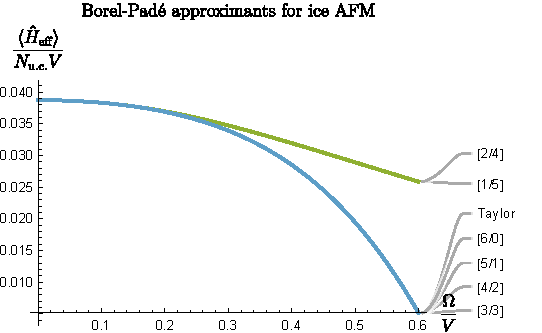
\includegraphics[width=\textwidth]{borel_pade_IAFM.pdf}
%          \caption{Ice antiferromagnet}
%          \label{fig:borel_pade_IAFM}
%      \end{subfigure}
%      \hfill
%      \begin{subfigure}[b]{0.45\textwidth}
%          \centering
%          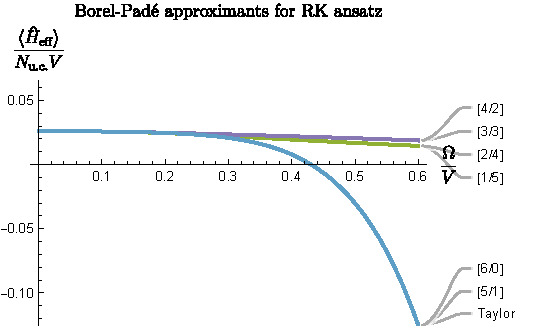
\includegraphics[width=\textwidth]{borel_pade_RK.pdf}
%          \caption{RK wavefunction}
%          \label{fig:borel_pade_RK}
%      \end{subfigure}
%      \begin{subfigure}[b]{0.45\textwidth}
%          \centering
%          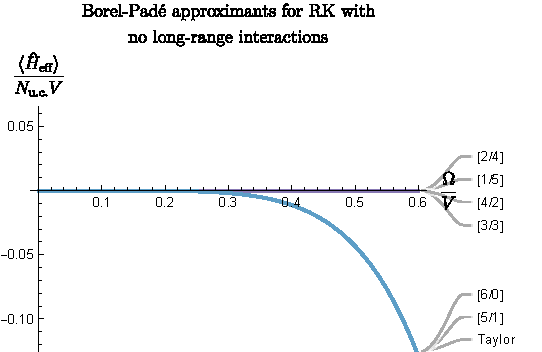
\includegraphics[width=\textwidth]{borel_pade_RK_noLR.pdf}
%          \caption{RK wavefunction with long-range interactions turned off}
%          \label{fig:borel_pade_RK_noLR}
%      \end{subfigure}
%         \caption{\response{Sub-figures (a), (b) and (c) show the various Borel-Pad\'e approximants and the Taylor series for the three ansatz states: ice ferromagnet, ice antiferromagnet and the RK wavefunction. Sub-figure (d) shows the Borel-Pad\'e approximants and the Taylor series for the RK wavefunction without the long-range interactions. The curves labelled ``Taylor" are the energies of the ansatz states obtained from perturbation theory. The curves labelled by ``$[m/n]$" where $m, n \in \{0,1,  ..., 6\}$ such that $m+n=6$ are the $[m/n]$ Borel-Pad\'e approximants.}}
%         \label{fig:borel_pade}
% \end{figure}








% -----------------------------------------------------




\item \textit{In his 1956 paper (Ref. [67] Phys. Rev. 102, 1008 (1956)), Anderson
studied the problem of charge ice in magnetite and the role of the
long-range Coulomb repulsion. He figured out that one can follow the
Madelung method to minimize the Coulomb energy. As a result, one
divides the lattice into neutral lines of atoms where the charges are
arranged alternatively (ABABAB...) so that the potential falls off
rapidly with the distance from a line. A similar result was obtained
for the spin ice, where the spin interacts by the long-range dipolar
interaction [Phys. Rev. B 92, 094418 (2015)]. Would such an ordering
principle also work for the van der Waals interactions?
}

%\commentGN{We need to understand Anderson's paper. Nevertheless, our result is exact. So understanding Anderson's argument may help provide more intuition to our result but not much else.}


\response{Our response: The ferromagnet phase described in the 2015 paper mentioned by the Referee (Ref.~\cite{mcclarty2015chain}) is the same as the ice FM in our manuscript. Thus, the ice FM can also be thought of as composed of alternating chains of spins and follows the ordering principle of Ref.~\cite{mcclarty2015chain}.
In Ref.~\cite{mcclarty2015chain}, the division of the lattice into neutral lines of atoms with alternating charges was useful because it allowed the authors to map their (classical) system to an Ising model and find the ground state in a range of parameters where the Luttinger-Tisza method could not.
Since the Luttinger-Tisza method gives the ground state of our model in the classical limit ($\Omega =0$), we do not need an analysis similar to Ref.~\cite{mcclarty2015chain}.
Such an analysis will also show that the ground state is ice FM for $\Omega=0$. 
Thus we expect that the ordering principle of Ref.~\cite{mcclarty2015chain} will also work for our Hamiltonian, which has van der Waals interactions. We have added the following sentence at the end of Sec.~III~A~2.}

\wesay{We note that ice ferromagnet is one of the ``chain states" that were described in Ref.~\cite{mcclarty2015chain}.}

\textit{And what would
be the perturbational energy for the allowed states that follow this
principle?}

\response{Our response: In Ref.~\cite{mcclarty2015chain}, the classical Hamiltonian, $\mathcal{H}_{\text{DSI}}$ shown in their Eq.~(7), has a free parameter $J_2/D$ which is the ratio of the next-nearest-neighbor exchange coupling to the dipole interaction strength.
Depending on $J_2/D$, they find various ordered states consistent with their ordering principle. 
Since our classical Hamiltonian does not have any free parameter, we obtain only one allowed state (ice FM) whose perturbational energy we had already calculated. In principle, one could consider a model with van der Waals interaction and an additional next-nearest-neighbor exchange coupling $J_2$, in which the ratio of $J_2$ to the van der Waals interaction strength can be varied. For such a model, it seems plausible that the ground states (in different regions of the parameter space) will be ice rule obeying states. We say this because, for the dipolar interaction of Ref.~\cite{mcclarty2015chain}, the ground states obeyed the ice rule and van der Waals interactions are weaker than dipolar interactions. If this is the case, then the mapping to a 2D Ising model with local interactions of Ref.~\cite{mcclarty2015chain} should also work for the van der Waals interaction.
% there could be more than one states following the ordering principle of Ref.~\cite{mcclarty2015chain}.
We find it an interesting direction to pursue, however that is not the focus of our manuscript. We have added the following sentences at the end of Sec.~III~A~2.}
\wesay{We here point out an interesting question: if we add a next-nearest-neighbor $\hat{S}^z\hat{S}^z$ interaction to $\hat{H}_{\text{cl}}$, do the ground states of this new Hamiltonian satisfy the ice rule and are they also ``chain states" as described in Ref.~\cite{mcclarty2015chain}? We leave it for future work to answer this question.}

\item \textit{To conclude, the phase diagram presented in Sec. III is anticipated
from the literature, and while it is sound, it is not necessarily the
final one - a more detailed numerical study would have been desirable
to confirm its validity. }

\response{We agree that a more detailed study is needed to get the final phase diagram. However, we think the work needed for such a numerical study deserves its own manuscript as we say in our response to point 3 above. To emphasize this point, we have added the following sentence right before  Sec.~III~B~1:}
\wesay{We note that, to be certain about the existence of all the phases we found and about not missing any additional phases, a more detailed quantum Monte Carlo study is required, and we leave it for future work.}

\item \textit{The concepts and suggested experimental
protocols for detecting spin liquid, outlined in section IV, would
merit acceptance in Phys. Rev. X if they were discussed in greater
depth and their usefulness shown satisfactorily using the model.
Overall, Section IV is difficult to read. For example, the steps from
Eq. (48) to Eq. (50) may be more explicit. At the same time, much
space has been devoted elsewhere to describing more straightforward
ideas; the article should be more balanced.}

\response{Our response: We are again happy to note that the Referee believes our manuscript  would merit acceptance in Phys.~Rev.~X if section IV was more detailed. As we already mentioned in response to point 4 above, based on Referee's feedback, we have significantly expanded Sec.~IV. In particular, we now explain the behavior of each correlator in each part of the phase diagram. We believe that the added details and intermediate steps have now made Sec.~IV easier to read. As an example, now the steps from Eq.~(55) (Eq.~(48) in the old manuscript) to Eq.~(66) (Eq.~(50)  in the old manuscript) are explicit. With the additions to Sec.~IV and some removal/shortening of sentences in Sec.~II after Eq.~(6) and Eq.~(8) and in the first paragraph of Sec.~II~A, we hope that our article is more balanced now.}

\item \textit{Some minor comments:}

\textit{(i) In Eq. (14), using $n_{rr'}$ and $\theta_i$ (i.e., two different types of
indices to denote the same sites) is confusing. Could one use the same
notation for both (e.g., $n_{rr'}$ and $\theta_{rr'}$)}

\textit{(ii) In Eq. (48), the "b"s are not the bosons "b" in Eq. (1), but the local
magnetic fields of the curl of "a" in Eq.(17) [it is confusing at
first]. One could define the "b" earlier [e.g., after Eq. (17) ].}

\response{Our response: We thank the Referee for these suggestions. We have incorporated both of them in our revised manuscript. More specifically, in Eq.~(14), we have changed the notation from $\hat{\theta}_i$ to $\hat{\theta}_{\vb{r}\vb{r'}}$.
We have also changed the notation for the magnetic field operator to ``$\hat{B}$" so that it is not confused with the bosons, ``$\hat{b}$". We also have defined $\hat{B}$ earlier after Eq.~(17) by adding the following sentence:}
\wesay{ Such a plaquette can be uniquely defined by $(\dual{r}, \mu)$, where $\dual{r}$ belongs to the dual lattice and $\dual{u}_\mu$ for $\mu \in\left\{1,2,3,4\right\}$ gives the plaquette orientation [as defined in Fig.~1(c)], and $\hat{B}_{\dual{r}, \mu}$ is the magnetic field operator at that plaquette.} 


\end{enumerate}

\noindent\makebox[\linewidth]{\rule{\textwidth}{0.4pt}}


\section{Response to Third Referee}
\begin{enumerate}
    \item \textit{In their manuscript, Shah and coworkers present a theory proposal for
the realization of quantum spin ice dynamics in Rydberg atom quantum
simulators. The backbone of the proposal is to utilize Rydberg
interactions to engineer strong constraints on the pyrochlore lattice,
so that a finite Rabi frequency generates `magnetic' fluctuations and
establishes a deconfined phase at sufficiently large coupling
(competing with long-range interactions). The authors utilize
perturbation theory and gauge-mean-field theory to describe the
transition from ordered to deconfined, and from deconfined to Higgs.
Both state preparation and diagnostics of the various phases are
discussed, including comments relevant to experimental feasibility.}

\textit{Overall, the work is very well structured, and clear. What I
appreciated the most is the attention to diagnostics, a very important
element for such strongly correlated and non-trivial phases, that is
often neglected in theory proposals. The section on monopole operators
is particularly informative.}

\response{Our response: We thank the Referee for going through our manuscript, providing insightful suggestions and comments some of which we missed noticing. We are happy to hear that the Referee found our work well structured, clear and having content that is often neglected in theory proposals.}

\item \textit{Novelty of the approach and results: from the point of view of
technical novelty, the paper is rather standard. The implementation
part, that is the one with the expected wider impact, combines
techniques proposed in [51] and Rydberg works - [63, 64] and others on
frustrated Ising magnets (including Lukin's experiments), and others
[98-99] working with XY magnets. Also, the connection between abelian
gauge theories and Rydberg interactions is very well known, so in that
context, the present work is construed as another promising example
along an established route. Finding a gauge theory dynamics that has
deconfinement in similar situations is, if not expected, quite likely
based on earlier results.}

% \response{Our response: While it is true that our work heavily relies on existing results in the literature,  examining the stability of the QSL in the presence of long-range interactions by sixth-order perturbation theory goes significantly beyond the existing literature.
% Furthermore, the behavior of the correlators in various phases and the protocols to measure them in Sec. IV add novelty to our manuscript.  
%Some of these results are more fundamental.
%For example, the numerical calculation of the plaquette correlator for the Rokhsar-Kivelson wavefunction has never been done before and is a more general result (independent of the specific kind of interactions).
%  Since we have significantly expanded Sec.~IV of our manuscript, we would invite the Referee to reconsider the novelty of our results. 
% Please see our response to point 5 below as well. \commentJS{Is this a good response?}
% }

\response{Our response: While it is true that our work relies heavily on existing literature, we believe that our work goes significantly beyond the existing literature for the following reasons:
\begin{enumerate}
\item The entire search for a system whose state is in the $U(1)$ quantum spin liquid phase has been restricted to traditional condensed matter systems so far. We are pointing out a novel direction for the search of a $U(1)$ QSL.
\item Furthermore, the main diagnostic in these traditional condensed matter systems are the pinch point singularities in correlation functions of certain local operators. The monopole correlator which we propose to measure is the expectation value of a non-local operator. This contributes to the novelty of our manuscript.
\item Analyzing the effects of long-range van der Waals interactions on the stability of a QSL using sixth-order perturbation theory had not been considered before in the literature.
\item While the connection between Rydberg atom arrays and Abelian gauge theories in 1D and 2D has been studied in depth in the literature before, 3D has remained completely unexplored. It is well-known that gauge theories in 3D behave very differently than those in 2D. For example, compact $U(1)$ gauge theory in 2+1D is always confining (by Polyakov’s argument~\cite{polyakov1977}), while compact $U(1)$ gauge theory in 3+1D can be either in the confined or the deconfined phase depending on the coupling. Since the paper by Semeghini et.~al.~in 2021, numerous proposals for realizing quantum spin liquids in 2D have come up (Refs.~\cite{tarabunga2023classification, slagle2022quantum, kornjaca2023trimer, ohler2023quantum}). However, there is not a single proposal about QSLs in 3D. Thus our work is the first step in a direction which is unexplored in literature. 
\end{enumerate}
To emphasize these points in our manuscript, we have added the following sentences in the second, third and last paragraphs of the introduction (Sec.~I):
}
\wesay{\textcolor{black}{$\dots$ has sparked a lot of activity over the past few years in the general direction of proposing ways to realize exotic states on quantum devices using analogue quantum simulation~\cite{myerson2022construction,slagle2022quantum, giudice2022trimer,zhou2022quantum, tarabunga2023classification, kornjaca2023trimer,ohler2023quantum}, digital quantum simulation~\cite{liu2021methods}, and projective measurements~\cite{tantivasadakarn2022shortest,verresen2021efficiently}.} However, all of these proposals have been for two-dimensional Rydberg-atom arrays.}
\wesay{With our proposal, we intend to push the search for a $U(1)$ quantum spin liquid, which has traditionally remained limited to solid state systems, in the direction of three-dimensional Rydberg atom arrays.
The connection between Rydberg-atom arrays and Abelian gauge theories in one dimension and two dimensions has been studied in depth in the literature before~\cite{cheng2024emergent, ohler2022self, surace2020lattice, cheng2023gauge}; however, this connection in three dimensions has remained unexplored. It is known that gauge theories in three dimensions can have a significantly different behavior than those in two dimensions. This is illustrated by the compact $U(1)$ gauge theory.
% in 2+1D is always confining (by Polyakov’s argument~\cite{polyakov1977}), while compact $U(1)$ gauge theory in 3+1D can be either in the confined or the deconfined phase depending on the coupling.
}
\wesay{\textcolor{black}{In Sec.~IV, we present correlation functions that distinguish the spin liquid from the ordered phases.} We explain the behavior of the correlation functions in each phase of the phase diagram. We also provide protocols to measure them.}

\response{We have significantly expanded Sec.~IV of our manuscript by adding subsections explaining the behavior of each correlator in each phase of the phase diagram. Furthermore, we have rewritten Appendix~C (Appendix~B in the old manuscript) for better clarity and added a new Appendix, Appendix~D.}

\item \textit{The second most relevant result, in my opinion, is the classical
stability of ice rule in the presence of LR interactions. This result
is indeed interesting, but I do not find it groundbreaking. For
instance, the fact that the ice manifold can be remarkably robust to
LR interactions has been known since a while, even for interactions
that are much stronger than the ones used here. One example on - I
believe - the very same lattice discussed here, and dipolar
interactions, is Phys. Rev. Lett. 95, 217201 (2005), but there are
other recent works in classical statistical mechanics that illustrate
that (on different lattices). It ultimate significance to the quantum
case is also affected by the point below.}

\response{Our response: We agree with the Referee that the classical stability of the ice rule in the presence of long-range interactions is not groundbreaking.
However, it is important to study the effects of long-range interactions because, in the system of Ref.~\cite{semeghini2021}, long-range interactions were found to destabilize the QSL~\cite{verresen2021}.
We would like to emphasize that it is also not the focus of our work, but just one intermediate result. }

\response{We thank the Referee for pointing out the 2005 PRL. We have cited it (Ref.~[85]) 
%and written a few sentences about the stability of the ice manifold under dipolar interactions right before Sec. III.
and written the following sentences right before Sec.~III.}

\wesay{While these works suggest that long-range interactions could destabilize the quantum spin liquid and favor an ordered state, it is not always the case as was discovered in Ref.~\cite{isakov2005why}, where the degeneracy of the ice manifold was preserved despite the introduction of a dipolar-like long-range interaction. Thus, in our work, it is important to study the effects of the van der Waals interaction more closely.}

\item \textit{Validity of the quantum treatment: The few body discussions are very
solid, and I could not spot any clear weakness there (apart from the
accurate determination of certain operators in terms of mapping from
field theory to lattice, which is of course quite hard in general).
The many-body treatment carried out by the authors is instead not
state of the art. Rather controlled (Green function) Monte Carlo have
been routinely performed on similar models since 2010's, by several
groups (Shannon, Pollman, Moessner, etc.). The perturbative approach
the authors carry out can be at most a qualitative guide (as the
authors fairly acknowledge in the conclusions), which is somehow
problematic given that most physics seems to appear at $\Omega$ of order
1, where perturbation theory is not likely to be accurate. So, the
phase diagram is yet to be solidly established.}

\response{Our response: We agree with the Referee that a Green function Monte Carlo can be done (especially since our Hamiltonian does not have the sign problem) and will give an accurate phase diagram. However, we believe that such a calculation deserves its own manuscript.
% as mentioned in our response to point 3 made by Referee 2. 
To emphasize this point, we have added the following sentence before the beginning of  Sec.~III~B~1:}
\wesay{We note that, to be certain about the existence of all the phases we found and about not missing any additional phases, a more detailed quantum Monte Carlo study is required, and we leave it for future work.}

\response{We have addressed the point about the convergence of the perturbation series by calculating the Borel-Pad\'e approximants in the new Appendix~A. The analysis in this Appendix shows that, if we were to use Borel-Pad\'e approximants for the energies of the ice FM and ice antiferromagnet states instead of their Taylor series, while using the Taylor series for the RK wavefunction, the phase diagram would change only slightly. That is, the critical coupling between the ice FM and the QSL phases would change from $\Omega_C = 0.43927 V$ to $0.44067 V$. We don't use the Borel-Pad\'e approximants for the RK wavefunction because we find that they do not capture the energy decrease coming from quantum fluctuations completely as we explain in the Appendix. This analysis has increased our confidence in the phase diagram being correct qualitatively. We have added the following sentences to the manuscript based on this point (Sec.~III~A~4, second-to-last paragraph):}
\wesay{In Appendix~A, we address the issue of the convergence of the perturbation theory by calculating the Borel-Pad\'e approximants of the perturbational energies of the three ansatz states. We find that using the Borel-Pad\'e approximants for the ice FM and the ice antiferromagnet does not change the phase diagram qualitatively.}
%in our response to point 6 of Referee 2. 

\response{However, in case the true phase diagram turns out to not have a QSL phase, the interaction can be modified by ``dressing" the atoms. 
In the technique of Rydberg dressing~\cite{hines2023spin}, an off-resonant laser hybridizes the ground state with a Rydberg state. Doing so modifies the form of the effective interaction between Rydberg atoms. We have mentioned this in the second paragraph of the Discussion section. By choosing the excited state and the strength of hybridization appropriately, one 
 could potentially reduce the destabilizing effect of long-range interactions. One can also dress the atoms so that the interactions are strongly peaked in distance~\cite{hollerith2022realizing, steinert2023spatially}. Using this technique, one could potentially make the nearest-neighbor interaction much stronger than interactions at larger distances and thereby  enlarge the QSL region in the phase diagram. We have added the following sentence in the second paragraph of the discussion in relation to this point:
 \wesay{It is also possible to engineer interactions that are strongly peaked in distance~\cite{steinert2023spatially, hollerith2022realizing} which could allow the nearest-neighbor interactions to be much stronger than the interactions at other distances, and potentially make the QSL more stable.}}
 
\response{Moreover the dynamical state preparation protocol does not require one to have the ground state be in the QSL phase. We have argued that it prepares a state with large overlap with a QSL state even if the ground state is an ordered state in Sec~III~C. 
%In such a scenario, all the measurement protocols and the concepts of Sec. IV would still be valid and useful. 
It was actually the case in the experiment in Ref.~\cite{semeghini2021} that the true ground state was not a QSL, but their sweeps of parameters were such that a state with a large overlap with the RVB state was prepared.   We have added the following sentence right before the beginning of Sec.~IV in the manuscript to  emphasize this point. The ``first method" here refers to the dynamical state preparation method.}

\wesay{We note that the first method above can prepare a state with a large overlap with the RK wavefunction even if the true ground state of the system is not in the QSL phase.}

\item \textit{Based on my comments above about novelty of the approach, of the
results, and validity of the quantum treatment, I feel that the work
shall be publishable, but it does not meet PRX criteria of a
fundamentally new, exciting, and a highly key contribution to the
current studies in the field of frustrated quantum magnets. The work
is a - solid and appreciated - continuation of a successful research
line connecting Rydberg dynamics and abelian gauge fields.}

% \response{Our response: Sec.~IV has been significantly expanded, and we urge the Referee to reconsider their decision. 
% \commentJS{Is it okay to say this?}
% We would like to emphasize that we are pushing the search for a $U(1)$ quantum spin liquid which has remained restricted to traditional condensed matter systems, in the direction of Rydberg atom arrays. With our proposal we are also pushing the established field of quantum simulation in 2D Rydberg atom arrays to 3D arrays which has remained largely unexplored in the literature. 
% While the connection between Rydberg dynamics and Abelian gauge fields in 1D and 2D has been well studied, 3D has not been considered before. 
% Moreover, Abelian gauge theories in 2D can be very different than those in 3D. For example, the $U(1)$ gauge theory in 2+1D is always confining by the Polyakov argument, while the $U(1)$ gauge theory in 3+1D has a deconfined phase.
%  3D gives access to new phenomena.
% Thus, our manuscript satisfies the PRX acceptance criterion of ``Push an established field into a new direction."}
\response{Our response: As we said in our response to point 2 above, the search for a $U(1)$ quantum spin liquid has remained restricted to solid state systems and we are pointing out a new direction for this search. Furthermore, the proposals to realize a QSL using Rydberg atom arrays have so far been restricted to 2D. Our manuscript is the first proposal of a quantum simulation experiment involving 3D Rydberg atom array in optical tweezers. If a $U(1)$ QSL is indeed realized in such an array, then it will be a breakthrough. Thus we believe that our manuscript satisfies the following PRX acceptance criterion: ``Push an established field into a new direction." Furthermore, we reiterate here that while the connection between Rydberg atom arrays and Abelian gauge theories in 2D and 1D has been studied in detail in the literature, the connection in 3D has remained unexplored. Our response to point 2 above lists the changes we made in the text to emphasize all of these points.}


\response{Using our proposal, both the deconfinement-confinement and the Higgs transitions of the compact $U(1)$ gauge theory can be accessed by changing the ratio of the Rabi frequency to the van der Waals interaction strength. We have added the sentence shown below to emphasize this point in the last paragraph of the introduction. These transitions are of interest in both high-energy physics and condensed matter physics. Therefore, our work is a fruitful connection between condensed matter physics, AMO (atomic, molecular, optical) physics,  and high-energy physics. Thus, we believe we satisfy the following PRX acceptance criterion: ``Establish a fruitful analogy or connection between different sub-fields or topical areas of physics, or between physics and other scientific disciplines."}

\wesay{Thus both the deconfinement-confinement and the Higgs transitions of the compact $U(1)$ gauge theory can be accessed by changing the Rabi frequency in our model.}
\item \textit{I have some minor comments that I believe could help the authors
ameliorate their already nice to read manuscript:}

\textit{- References 64 and 76 are identical;}

\textit{- in page 6, when discussing even/odd effect, it might be useful to
draw a parallelism with the Schwinger model, where even/odd is related
to background potentials and leads to the same type of frustration the
authors mention (I found their explanation rather clear, but the
Schwinger model parallelism is likely better known in the particle
physics community);}

\response{Our response: We thank the Referee for these comments, and we are happy to note that the Referee found our manuscript nice to read. We have removed one of the references and have added the following sentence in the first paragraph of the right column on page 6.}
\wesay{For readers familiar with the Schwinger model, we point out that the even and odd compact $U(1)$ gauge theories are reminiscent of gauge theories with a $\theta$-term in $1+1$ dimensions at $\theta=0$ and $\theta=\pi$, respectively.} 



\item \textit{In page 7, one shall cite Sondhi's et al., Phys. Rev. Lett. 95,
217201 (2005) - that emphasize how, in general, long-range
interactions do not destabilize a deconfined phase, and can actually
make it more robust. Of course, truncating interactions might favor
order, but this is very much truncation dependent.}

\response{Our response: We thank the Referee for pointing out this interesting work. We have added this reference (Ref.~[85] in the manuscript) and written the following sentences
% about the stabilization of the QSL in presence of certain long-range interactions 
at the end of Sec. II C as we mention in our response to point 3 above.}
  \wesay{While these works suggest that long-range interactions could destabilize the quantum spin liquid and favor an ordered state, it is not always the case as was discovered in Ref.~\cite{isakov2005why}, where the degeneracy of the ice manifold was preserved despite the introduction of a dipole-like long-range interaction. Thus, in our work, it is important to study the effects of the van der Waals interaction more closely.}

\item \textit{ What the authors refer to as BFFM makes not much sense to me. BF and
FM are (a) two distinct operators - in fact, FM works criticized BF
operator and showed that it is not related to confinement, but rather,
to other spectral properties, and (b) are defined in imaginary time,
while here, the authors consider them as real space operators. Since
Lorentz invariance is not present here, it is unclear if a real-space
only operator has a direct relation to the operators above. So I have
two questions:}

\textit{A) What are the authors measuring? the real space version of BF or FM
operators? can they elaborate on this? Have they discovered some
unexpected equivalence between the two? in case so, could they point
out discrepancy in the previous analysis of FM?}

\response{Our response: Our reason for calling the correlator that we measure as BFFM was because this name was used in the arXiv version (but not in the published version) of the work by Semeghini et al. (Ref~\cite{semeghini2021probingarXiv}). %Ref.~\cite{semeghini2021}, 
however after taking a deeper dive into the literature (Refs.~\cite{fredenhagen1983charged, fredenhagen1986, fredenhagen1988dual, bricmont1983order}), we agree with the Referee that BF and FM are distinct operators. 
One difference being this: BF does not involve closed loop operators while FM involves closed loop operators in the denominator. 
We are proposing to measure the real space version of the FM operator and we have changed BFFM to Fredenhagen-Marcu at all places in our manuscript (we do not use the abbreviation FM for Fredenhagen-Marcu since we already use this abbreviation to denote a ferromagnet).}

\textit{B) In case the authors indeed study the real space FM operator, why do
they expect that the latter behaves like its original version? Clear
evidence of this must be provided.}

\response{Our response: In the original work by Fredenhagen and Marcu (Ref.~\cite{fredenhagen1983charged}), they came up with the space-time version of the FM operator and in their subsequent work~\cite{fredenhagen1988dual}, they also argued that the real-space version can be used to diagnose deconfinement. In particular, in Sec. 5 B of ~\cite{fredenhagen1988dual}, they propose the real-space version. 
In the context of condensed matter physics,   Ref.~\cite{gregor2011diagnosing} showed that the real space FM operator can be used as a diagnostic for deconfinement for both the $\mathbb{Z}_2$ and compact $U(1)$ gauge theories with matter. 
%and show that both the imaginary time and the real space version of the FM operator can distinguish a confined from a deconfined phase. 
In their Sec 8.3 they note that the real space version of the FM operator can be used to detect phases of dimer models with gapped spinons, which is similar to our situation.
The real space version has also been used in recent works \cite{semeghini2021, verresen2021, gregor2011diagnosing, xu2024critical} to diagnose deconfinement. We believe there is plenty of literature that supports that the real space FM operator can diagnose a deconfined phase.}

\response{We have clarified this point in the first paragraph of Sec.~IV~C (above Eq.~(82)) in a few sentences 
% above Eq.~(82) in the revised manuscript that we are using the real-space version of the Fredenhagen-Marcu order parameter. 
We have also cited Refs.~\cite{fredenhagen1988dual, verresen2021, xu2024critical, gregor2011diagnosing} there. These are the sentences we have added:}
 \wesay{In its original formulation~\cite{fredenhagen1983charged}, the Fredenhagen-Marcu order parameters involved expectation values of operators in space-time. Subsequently, real-space versions were proposed and studied~\cite{fredenhagen1988dual,gregor2011diagnosing,verresen2021,xu2024critical}. We will be using the real-space version of the Fredenhagen-Marcu order parameters here.}

%\commentGN{We need to answer this seriously. We are considering an equal-time version. Lukin + Ashvin's papers also considered similar correlators at equal time.}

\item \textit{When citing state preparation, it might be worth to cite PRL 129,
090401 (2022) on how state preparation can actually enlarge spin
liquid regions (or, more precisely, enlarge finite size overpals with
RK-like wave functions).}

\response{We thank the Referee for pointing out this paper. We have cited it in the first paragraph of Sec.~III~C and added the following sentences about it.}
\wesay{In the context of the experiment in Ref.~\cite{semeghini2021}, it was shown numerically in Ref.~\cite{giudici2022dynamical} 
that a state with a large overlap with the RVB state can be prepared by a non-equilibrium time evolution.}


\item \textit{I have not really understood the graphics in Fig. 13 b. I am
unfortunately unable to provide any constructive criticism here [I
found instead the other graphics in 13c clear enough], so I leave to
the authors any choice about revising that;}

\response{We are sorry to hear that Fig.~13(b) was not clear enough to understand. We have added more details to the caption of Fig.~13(b). It shows the side view of the configuration in Fig.~13(c). We think it is illuminating to add Fig.~13(b) because the 3D lattice might be difficult to visualize based on just Fig.~13(c). To make the configuration clear, we are submitting a 3D animation as a Supplementary Material item with the name ``Monopole Gauge Field Configuration.mp4". We have referenced it in the caption of Fig.~13. Some of the additions to the caption of Fig.~13 are}
\wesay{\textcolor{black}{(b) A side view of the stack showing three of its layers, }where each layer is made of 7 puckered hexagons of the diamond lattice. The bonds within each of these layers are colored in yellow, orange, and cyan. The bonds (of the diamond lattice) connecting sites of two different layers are shown in black. $\dots$ The two sub-lattices of the diamond lattice are represented by blue and green sites. $\dots$ See also Supplementary Material for an animation showing other points of views~\cite{supp}.} 


\item \textit{Not clear immediately clear to me how Eq. 62 is informative. It is
likely to work only deep in the confined phase, as there is a large
discrepancy as a function of $\Omega$. The authors acknowledge this at
the end of the subsection, but I do not fully understand why they
claim this is still relevant (the puddles will be too small to observe
an asymptotic behavior I believe). 
}

% \response{Eq. 62 of the old manuscript defines an operator $\tilde{\chi}_{\mathcal{C}}^E$ which is equal to the FM order parameter, $\chi_{\mathcal{C}}^E$ for $\Omega \ll V$. For $\Omega \gg V$, ground state is in the transverse field polarized (TFP) phase the two quantities are not equal, however both approach a non-zero constant in the limit of large curves $\mathcal{C}$. This was not explained in the old manuscript but is now explained in Sec. IV C 3 of the new manuscript.}

\response{Our response: The quantity defined in Eq. (62) of our old manuscript (Eq.~(85) in the revised manuscript), $\tilde{\chi}_{\mathcal{C}}^E$, is equal to the Fredenhagen-Marcu order parameter $\chi_{\mathcal{C}}^E$ for $\Omega \ll V$.
If one prepares the QSL using adiabatic state preparation, then $\Omega/V$ at the end of the adiabatic sweep must be between $0.44V$ and $0.55V$ so that the ground state is a QSL.
In this region, the discrepancy between $\tilde{\chi}_{\mathcal{C}}^E$ and $\chi_{\mathcal{C}}^E$ will be large as the Referee writes. 
In this case, we do not expect $\tilde{\chi}_{\mathcal{C}}^E$ to be able to distinguish the QSL from the confined phase (ice FM). 
However, we think $\tilde{\chi}_{\mathcal{C}}^E$ is relevant in the case of dynamical state preparation with final $\Omega/V$ much smaller than 0.44. %where the final  $\Omega/V$ of the state preparation need not lie in $[0.44, 0.55]$ and can be quite small.
Puddles of QSL will be formed if one uses dynamical state preparation.
% However, we still think $\tilde{\chi}_{\mathcal{C}}^E$ is relevant if the state is prepared dynamically where puddles of QSL are formed.
% Because, in this case, the final  $\Omega/V$ of the state preparation need not lie between $0.44$ and $0.55$ and can be quite small.
The Referee is concerned that the puddles will be too small to observe the asymptotic behavior of $\tilde{\chi}^E_{\mathcal{C}}$. 
While we do not have estimates of the sizes of the puddles, the experiment in~Ref.~\cite{semeghini2021} on the 2D Ruby lattice suggests that it might be possible to see the change in the Fredenhagen-Marcu order parameter as one goes from inside the QSL phase to the outside of it. 
Note that, in their experiment, they employed a dynamical state preparation scheme and puddles of QSL were presumably formed.
Figuring out if the asymptotic behavior will be observable in an experiment requires one to estimate the sizes of the puddles which we think is beyond the scope of our manuscript.
To acknowledge the above point, we have added the following sentence at the end of the fourth paragraph of the Discussion section:}
\wesay{One must also estimate the size of the puddles of the QSL and compare them to the length scale at which the asymptotic behavior of the correlators is observed. We leave this for future work.}
\response{If future work shows that the puddles are too small to observe the asymptotic behavior, one can potentially modify the interaction to be sharply peaked at the nearest-neighbor distance by dressing the atoms~\cite{steinert2023spatially, hollerith2022realizing} so that the QSL regions extend for smaller $\Omega/V$ than for our current model. We have mentioned this in the manuscript in the second paragraph of the Discussion section. For ease of access, we rewrite those sentences here:
\wesay{\textcolor{black}{While it is possible that the true phase diagram differs from what we found, we note that there are other knobs one can tune to get a desired phase diagram. Dressed states created from multiple Rydberg and possibly ground levels can be used to customize the interactions away from the isotropic $1/r^6$ form we considered in this paper \cite{de2017Optical,glaetzle2015designing,van2015quantum,petrosyan2014binding,grass2018fractional,young2021asymmetric}.} It is also possible to engineer interactions that are strongly peaked in distance~\cite{steinert2023spatially, hollerith2022realizing} which could allow the nearest-neighbor interactions to be much stronger than the interactions at other distances, and potentially make the QSL more stable. \textcolor{black}{ Designing a dressing scheme compatible with the symmetries of the pyrochlore lattice and exploring the resulting phase diagrams is an interesting direction for future work.}}
Another possibility is to have $\hat{S}^z \hat{S}^z$ dipolar interactions between Rydberg atoms by either applying an electric field or dressing a Rydberg $s$ state with one or more Rydberg $p$ states~\cite{young2021asymmetric}. 
% Another possibility is to apply an electric field on the atoms so that the Rydberg atoms have an induced dipole moment and they interact via dipole-dipole interaction rather than van der Waals interaction.
% Another possibility is to use orbitals that have a dipole moment in optical tweezers so that the Rydberg atoms have  dipolar interactions between them.
% Another possibility is to use polar molecules in optical tweezers with dipolar interactions between them \commentJS{Alexey, could you check this sentence?}.
Dipolar interactions might have a less destabilizing effect than the van der Waals interaction because of Ref.~\cite{isakov2005why} which the Referee pointed out, and the QSL might extend for smaller $\Omega/V$. To emphasize this point, we have added the following sentences in the second paragraph of the discussion:}
\wesay{It is known that dipolar-like interactions can preserve the degeneracy of the ice manifold \cite{isakov2005why}. The QSL region can potentially be extended to smaller Rabi frequencies by making the Rydberg atoms interact via dipolar interactions either by applying a DC electric field or microwave-dressing a Rydberg $s$ state with one or more Rydberg $p$ states~\cite{young2021asymmetric}.}
% Another way to potentially have the QSL region extend to smaller Rabi frequencies is to apply an electric field so that the interaction between Rydberg atoms becomes dipolar~\cite{young2021asymmetric}.}


\end{enumerate}
\section{Summary of changes}

(The reference numbers here are not the same as the reference numbers in the revised or old manuscript.)
\begin{enumerate}
    \item Added sentences to the second, third and last paragraph of the introduction highlighting the novelty of our work.
    \item Shortened Section II by making the explanation concise. Specifically, removed sentences after Eqs.~(6),~(8), before Eq.~(7), and in the first paragraph of Sec.~II~A.
    \item Changed the notation in Eq.~(14) from $\hat{\theta}_i$ to $\hat{\theta}_{\vb{r}\vb{r}'}$. Also changed the notation for the magnetic field operator from $\hat{b}_{\dual{r},\mu}$ to $\hat{B}_{\dual{r},\mu}$ and introduced it after Eq.~(18).
    \item Pointed out the analogy of the even and odd compact $U(1)$ gauge theory with the Schwinger model on Page 6.
    \item Cited Ref.~\cite{isakov2005why} in Sec. II C and mentioned that certain dipolar like long-range interactions can not split the degeneracy of the ice manifold.
    \item Mentioned explicitly in Sec. III A 2 that we are using the Luttinger-Tisza method to calculate the ground state for $\Omega=0$ . Cited Refs.~\cite{luttinger1946theory, lyons1960method,litvin1974luttinger}.
    \item Cited Ref.~\cite{mcclarty2015chain} at the end of Sec.~II~A~2 and pointed out the ice FM is a ``chain state".
    \item Mentioned and summarized our Borel-Pad\'e analysis in the second last paragraph of Sec.~II~A~4.
    \item Acknowledged that a quantum Monte Carlo study is required to get the true phase diagram right before Sec.~II~B~1.
    \item Cited Ref.~\cite{giudici2022dynamical} in Sec. III C and commented on it. Added a sentence in the paragraph before the beginning of Sec.~IV.
    \item  The entire Sec. IV has undergone substantial changes. Sec. IV now spans around 9 pages while it spanned only 5.5 pages in our initial manuscript. A lot of explanation, new calculations and steps have been added. Some of these changes are:
    \begin{enumerate}
        \item Added subsections explaining the behavior of each correlator in each phase of the phase diagram.
        \item Changed the definition of the plaquette operators. For example the definition of the plaquette X operator was changed from a product of $\hat{S}^{\pm}$ to a product of $\hat{S}^x$ as these definitions  make the explanations clearer. Also changed from the disconnected plaquette correlators to the connected plaquette correlators.
        \item Entries in Table II were updated.
        \item Changed BFFM to Fredenhagen-Marcu everywhere in the manuscript. Clarified that we are using the real-space version above Eq.~(82).
        \item Added details to the  caption of Fig. 13. Submitted a 3D animation of the gauge field configuration.
    \end{enumerate}
    \item Added a few sentences to the second paragraph of the Discussion section about Rydberg dressing. Also added a couple of sentences in the fourth paragraph of the Discussion section about the size of the puddles of QSL.
    \item Added a new Appendix with our Borel-Pad\'e analysis.
    \item Changed the contents of Appendix~C (Appendix~B in the old manuscript) and added a new Appendix~D.
\end{enumerate}

\bibliography{rydbergs.bib}
\end{document}